% !TEX root = ../../main.tex
\subsection{安全性测试}

本节使用攻击演示脚本（\texttt{attack\_demo.py}）针对第三章定义的各类威胁场景进行安全测试。脚本包含 11 个场景（含 2 个正常操作基线），测试结果如表~\ref{tab:security_test}所示，完整运行输出如图~\ref{fig:attack_demo}所示。

\begin{table}[H]
\centering
\caption{安全性测试用例与结果}
\label{tab:security_test}
\small
\begin{tabularx}{\textwidth}{c l l X X c c}
\hline
\textbf{编号} & \textbf{攻击类型} & \textbf{威胁} & \textbf{攻击手段} & \textbf{预期防御} & \textbf{实际} & \textbf{结论} \\
\hline
S01 & 未登录创建订单 & T1 伪造 & 无登录态调用创建订单 & 401 拒绝 & 401 & ✓ \\
S02 & 伪造 Token & T2 伪造 & 修改 Token 末位字符 & valid=false & valid=false & ✓ \\
S03 & 跨用户越权 & T1 越权 & mallory 验证 alice 订单 & 403 拒绝 & 403 & ✓ \\
S04 & 未登录接单 & T1 伪造 & 无登录态调用接单 & 401 拒绝 & 401 & ✓ \\
S05 & 正常接单（基线） & — & 骑手首次接单 & 200 成功 & 200 & ✓ \\
S06 & 重复接单 & T6 滥用 & 同一骑手再次接单 & 400 拒绝 & 400 & ✓ \\
S07 & 管理员越权 & T6 越权 & 无登录态访问管理员接口 & 403+审计日志 & 403 & ✓ \\
S08 & 管理员登录（基线） & — & demo 账号登录 & 200 成功 & 200 & ✓ \\
S09 & hash-only 审计 & T7 隐私 & 管理员查看消息接口 & 无 content 字段 & 无 content & ✓ \\
S10 & 篡改检测 & T4 完整性 & 修改 DB 消息密文 & VERIFY\_FAIL & mismatch=1 & ✓ \\
S11 & 溯源滥用阻断 & T5 追责 & 调用明文关键词溯源 & 403 阻断 & 403 & ✓ \\
\hline
\end{tabularx}
\end{table}

\begin{figure}[H]
\centering
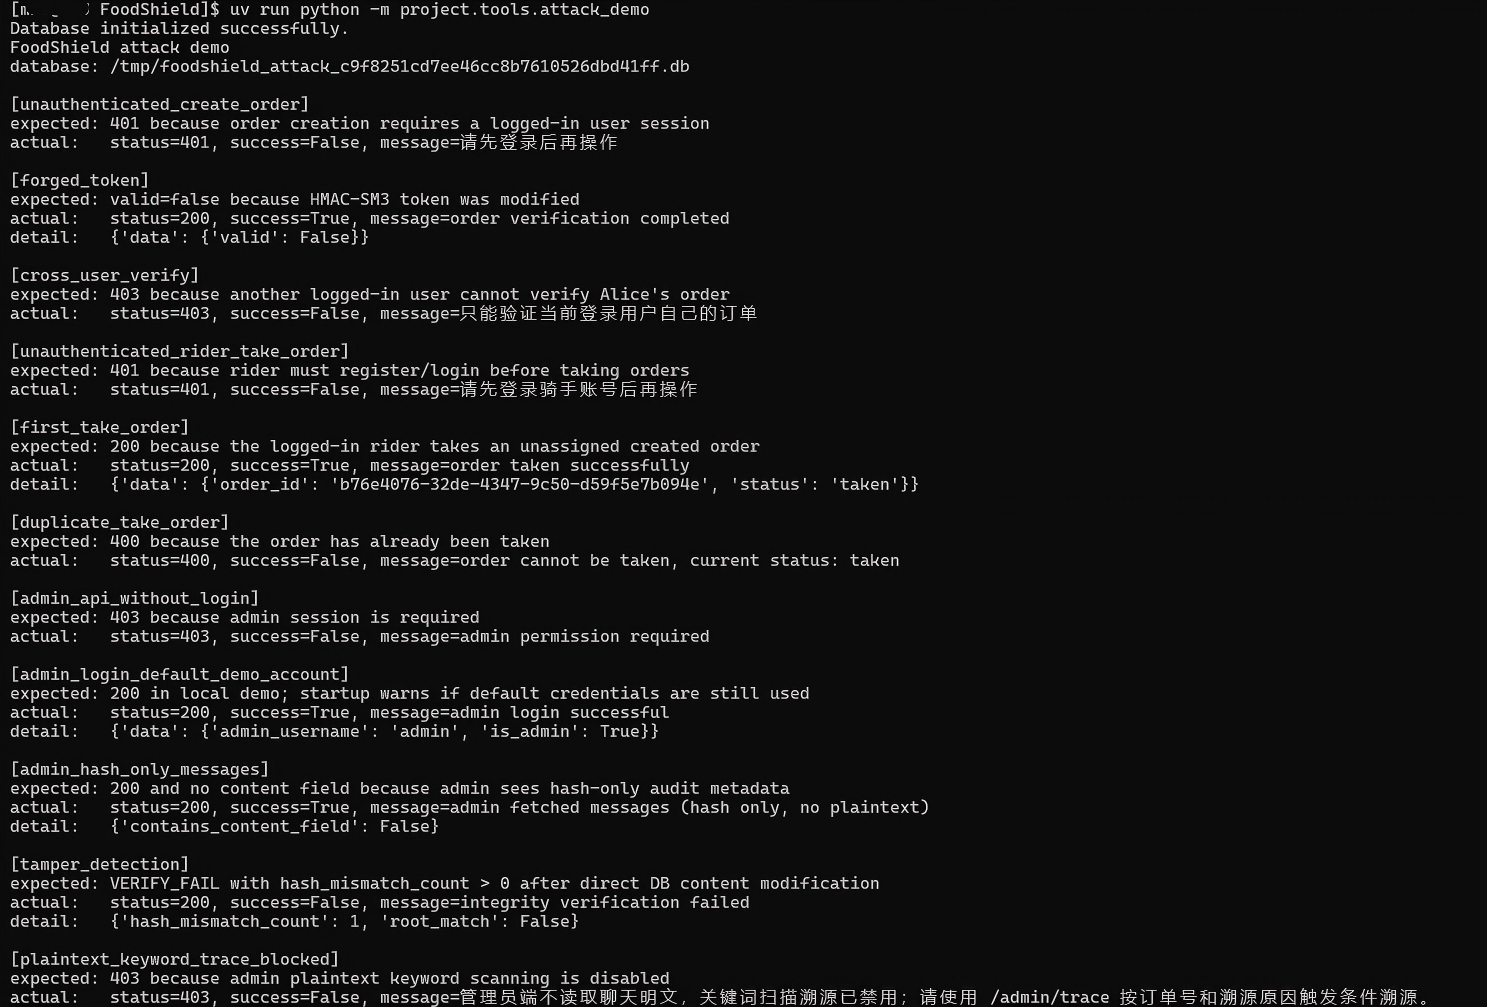
\includegraphics[width=0.95\textwidth]{content/chapter5/figure/attack_demo.png}
\caption{attack\_demo.py 运行输出（11 个场景全部通过）}
\label{fig:attack_demo}
\end{figure}

\textbf{S01--S02：身份与 Token 伪造}。无登录态请求被 \texttt{user\_required} 装饰器拦截返回 401；篡改 Token 末位后，\texttt{verify\_token} 重算 HMAC-SM3 发现不匹配，返回 \texttt{valid=false}，证明在未知$K_{\mathrm{order}}$下 Token 不可伪造。

\textbf{S03：跨用户越权}。后端从 session 获取当前用户 PID 与订单归属 PID 比对，不一致即返回 403，防止 Token 跨用户复用。

\textbf{S04--S06：骑手接单}。S04 验证未登录骑手被拒（401），S05 为基线（首次接单成功，状态 \texttt{created}$\to$\texttt{taken}），S06 验证重复接单被状态机拦截（400）。S05 的成功是 S06 拒绝的前提，两者共同证明接单状态约束有效。

\textbf{S07--S08：管理员访问}。S07 验证无管理员 session 时返回 403 并写入审计日志（action=\texttt{TRACE\_DENIED}），S08 为基线证明管理员认证流程正常。

\textbf{S09：hash-only 审计}。管理员消息接口返回数据仅含 \texttt{msg\_id}、\texttt{role}、\texttt{message\_hash} 和 \texttt{timestamp}，不含 \texttt{content} 字段，实现审计与隐私访问的接口级权限分离。

\textbf{S10--S11：完整性与溯源}。S10 验证篡改消息密文后完整性验证返回\texttt{VERIFY\_FAIL}（\texttt{hash\_mismatch\_count=1}，\texttt{root\_match=False}），详见 5.4 节。S11 验证管理员无法绕过审批流程直接扫描明文，溯源接口返回 403，溯源必须经完整性校验和审批双重门槛。
